\section{Implications of GPMs: Education, Safety, and Ethics}
\label{sec:implications}

The advent of \glspl{gpm} in the chemical sciences marks a paradigm shift that extends beyond methodological advances to fundamentally alter the conceptual frameworks through which scientific knowledge is produced and validated. 
As these models permeate education and research, their transformative potential is closely linked to critical challenges in cultivating discerning learners, mitigating emergent risks in automated discovery, and navigating ethical dilemmas arising from biased systems. 
Here, these tripartite implications are examined, and it is argued that responsible integration of \glspl{gpm} requires not only technical innovation but also rigorous pedagogical and regulatory frameworks.


\subsection{Education} \label{sec:education}

\subsubsection{Vision}

\glspl{gpm} are opening up new directions to create or use educational materials (see \Cref{fig:education}). 
Although many current applications are still in their conceptual stage, they begin to highlight the potential of these models to personalize learning, increase the fairness of evaluations, and improve accessibility. 
\glspl{gpm} can support both students and educators at various stages of the learning process and across different media forms, indicating a shift toward more adaptive and personalized educational frameworks. \autocite{Mollick2024}

For students, \glspl{gpm} could act as intelligent companions in a variety of tasks. 
As adaptive tutors, they could tailor explanations, exercises, and feedback to individual needs. 
Additionally, they could help students rehearse for exams and presentations and deepen their conceptual understanding. \autocite{mollick2024instructors, Sharma2025role, wang2025effect}

\begin{figure}[htb]
    \centering
    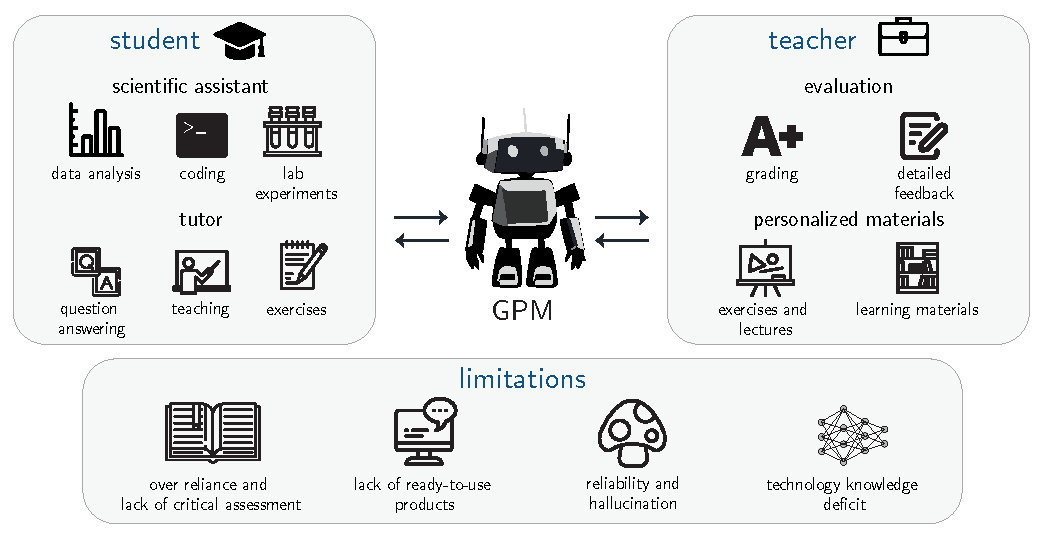
\includegraphics[width=1\linewidth]{figures/rescaled_figures/chemrev_figure23.pdf}
    \caption{\textbf{Possible application examples for students and teachers and their specific limitations for \glspl{gpm} in chemical education.} \glspl{gpm} can be used by students as scientific assistants (e.g., for data analysis, coding or lab experiments) and tutors (e.g., for question answering, teaching or exercises). Teachers can use \glspl{gpm} for evaluation (e.g., for grading and detailed feedback) or to personalize materials (e.g., for lectures and other learning materials). Current limitations include an over-reliance and a lack of critical assessment of the outputs, a lack of ready-to-use products, hallucination, a lack of reliability of the models, and a technology knowledge deficit of the users.}
    \label{fig:education}
\end{figure}

In more practice-oriented settings, such as laboratories or coding environments, these models could function as scientific assistants. They may provide real-time feedback on experimental setups, assist with how to use lab equipment, or help identify potential safety concerns.\autocite{Du2024} 
Coupled with \gls{ar}, \glspl{gpm} could also enable immersive simulations of lab procedures, allowing students to familiarize themselves with workflows and instruments before entering a physical lab. 
Moreover, by supporting students in technical areas such as coding, data analysis, or simulations, they could reduce the entry barrier or learning curve and thus foster interdisciplinary competence---particularly in contexts where instructor support is limited.

At the same time, \glspl{gpm} could ease the workload of educators. 
They offer new possibilities for generating and adapting course materials---ranging from lecture slides and exercises to individualized exam questions---thus enabling a better alignment with diverse learning levels and prior knowledge. In assessment tasks, these models could support the grading of open-ended responses by providing consistent, criteria-based feedback and reducing subjective bias.\autocite{Kortemeyer2024, gao2024towards} This is especially valuable in large courses or when timely, detailed feedback would otherwise be difficult to provide. 


\subsubsection{Current Status}

Despite these envisioned potentials of \glspl{gpm} in chemistry education, current applications are often still fragmented and lack integration into cohesive educational systems. 
In many cases, models are used via general-purpose interfaces without subject-specific customization or alignment with curricular goals. 
Rather than being part of purpose-built tools or platforms, their use remains largely exploratory.

\paragraph{General Systems}
Early applications often rely on zero-shot prompting of general-purpose \glspl{llm} or \glspl{vlm} to aid with student-oriented learning tasks. 
These include plotting data \autocite{Subasinghe2025}, writing code \autocite{Tsai2023}, or generating analogies to explain abstract chemical concepts \autocite{shao2025unlocking}. 

\textcite{handa2025education} analyzed over 570,000 anonymized Claude.ai conversations from university-affiliated users, finding that students primarily used the model for preparing learning materials ($39.3\%$) and solving academic problems ($33.5\%$). 
However, their use was often exploratory and low-stakes, and the study emphasizes the need for guidance, as many users lacked the expertise to evaluate model outputs critically.

Two recent studies have explored zero-shot prompting in more realistic, assessment-focused settings. \textcite{baral2025drawedumath0} introduced a benchmark of more than 2,000 student-drawn math images and found that state-of-the-art \glspl{vlm}, including \modelname{GPT-4o} and \modelname{Claude 3.5}, struggled to assess student reasoning and correctness, particularly in open-ended or diagram-based answers. 
Similarly, \textcite{Kortemeyer2024} investigated the use of \modelname{GPT-4} for grading handwritten thermodynamics exams at \modelname{ETH Zürich}. While the model performed reasonably well on short derivations, it failed to track detailed rubrics or interpret hand-drawn diagrams reliably. 
In chemistry education, \textcite{kharchenko2024advantages} compared \modelname{ChatGPT 3.5}, \modelname{Gemini}, and \modelname{Copilot} on domain-specific tasks and found that while the models performed adequately on simple recall questions, they failed in tasks that required chemical reasoning, structural understanding, or logical analysis.

Together, these findings suggest that while zero-shot prompting enables rapid deployment of \glspl{gpm} in educational contexts, current models lack the reliability, consistency, and domain grounding required for chemistry education---not only from a pedagogical standpoint, but also from ethical and legal perspectives.

\paragraph{Specialized Systems}
A growing number of applications embed \glspl{gpm} in specialized educational systems that combine \glspl{gpm} with structured components such as \gls{rag}, tracking learning progress, or the ability to work with multiple sources of content such as textbooks, lecture slides, or handwritten notes.

For example, \textcite{perez2025large} presented a biology \gls{qa} system that used a \gls{rag} pipeline to deliver curriculum-aligned answers. 
The I-Digest team \autocite{Jablonka2023} introduced a platform that generates lecture summaries and follow-up questions to support continuous learning. 
Some systems also integrate specialized components to improve personalization and continuity in the learning process. 
Although not designed for chemistry specifically, general-purpose platforms such as TutorLLM \autocite{li2025tutorllm0} (generating personalized content based on the learning progress) and LearnMate \autocite{wang2025learnmate0} (creating learning plans and giving feedback) demonstrate how large models can be embedded in structured educational frameworks. 

Anthropic's Claude for Education \autocite{AnthropicEducation} offers a purpose-built platform for higher education with a \enquote{Learning Mode} that uses the Socratic method to guide students rather than directly giving the answer to their queries. The intention here is to promote active learning and mitigate the risks of passive tool use. 
While such systems illustrate the potential of structured \gls{gpm}-based learning environments, fully integrated applications remain rare---particularly in domain-specific contexts such as chemistry. 
Furthermore, current models must still strengthen their robustness and domain-specific reasoning before they can be trusted in demanding fields, including chemistry.

\subsubsection{Outlook and Limitations}

While \glspl{gpm} offer promising opportunities for chemistry education, their use also raises critical ethical and pedagogical concerns.

A first concern is the lack of transparency in how these models generate responses. 
Although \glspl{gpm} produce fluent and plausible explanations, they do so without genuine understanding---and often with no clear indication of uncertainty or possible errors. 
This can lead students to accept incorrect or misleading information as fact, particularly when the output appears confident or authoritative. Over time, such interactions may normalize uncritical acceptance and discourage students from questioning, verifying, or reflecting on what they are told. 
In scientific education, where reasoning, skepticism, and an evidence-based mindset are essential, this poses a serious threat to the development of informed and independent   learners.\autocite{marcus2025will, kosmyna2025your}

A related but distinct issue is the risk of over-reliance and deskilling. When students delegate a large portion of the learning process to generative tools, they might be able to complete assignments without engaging in the mental work needed to develop subject-specific competence. 
In such cases, \glspl{gpm} can disrupt the connection between concrete tasks---such as solving a problem or writing an explanation---and the broader educational goals they are meant to support, such as developing chemical understanding or analytical thinking skills.\autocite{dung2025learning, Sharma2025role}

Today---and even more so in the future---students and learners will increasingly use \glspl{gpm}, both in education and in their future professions. 
Attempting to restrict their use is neither realistic nor educationally meaningful. 
Therefore, educators must guide their use thoughtfully and adapt both the learning process and assessment practices accordingly. 
Furthermore, the question of what to learn needs to be redefined. 
What we learn must increasingly center around the development of critical thinking, creativity, and logical reasoning---skills that remain essential and irreplaceable, even---or perhaps especially---in the age of \glspl{gpm}. \autocite{klein2025rethink}

\subsection{Safety} \label{sec:safety}

\begin{figure}[!htbp]
    \centering
    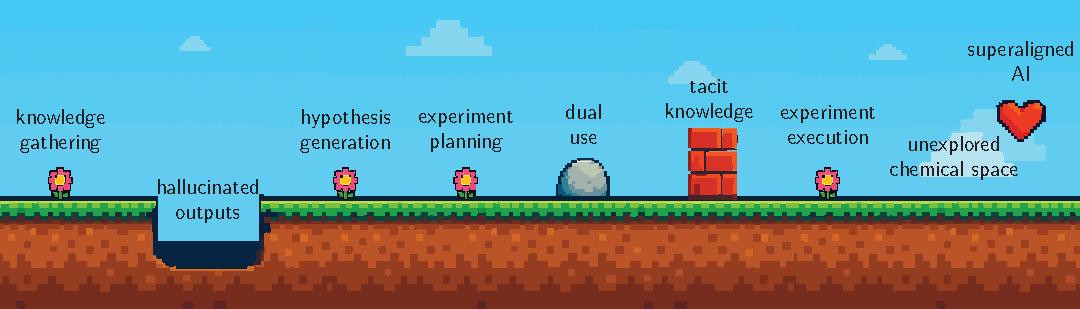
\includegraphics[width=1\linewidth]{figures/safety_chemrev_fig.pdf}
    \caption{\textbf{A conceptual schematic depicting \gls{ai} risk factors in chemical science}. As one traverses through the game-like scientific process, there are various obstacles to encountering \gls{ai} exacerbated risks. The path to superaligned chemical \gls{ai}-assistants is obfuscated by unexplored chemical space.}
    \label{fig:safety-overview}
\end{figure}

\noindent A growing coalition within the scientific community has sounded a call to action: \gls{ai} poses existential risks that deserve the same urgent attention as pandemics and nuclear war \autocite{cais2023statement}. 
This call, formalized in a statement signed by hundreds of prominent \gls{ai} researchers, reflects mounting recognition that advanced \gls{ai} systems could fundamentally alter, or threaten, human civilization. 
While the ongoing discourse has focused on abstract notions of \gls{agi}, the immediate risks may emerge through the integration of \gls{ai} into specific domains where the stakes are already high \autocite{morris2023levels}.

Chemistry represents one such domain. 
The rapid integration of \glspl{gpm} in chemistry is a dual-edged sword. 
Although these technologies can accelerate discovery, they also introduce unprecedented risks. 
From democratizing access to hazardous chemical knowledge to enabling autonomous synthesis of dangerous compounds, \gls{ai} systems could lower barriers for misuse, whether intentional or accidental. 
\glspl{gpm} alone may not create new risks \autocite{peppin2024reality}, but they can amplify existing ones (see \Cref{fig:safety-overview}).

Even in this amplified context, the ability of these systems to pose meaningful safety risks in practice is constrained by real-world limitations, including access to specialized lab equipment, regulated or scarce reagents, and, most critically, the \enquote{tacit knowledge}\autocite{Polanyi_2009} required to execute complex chemical processes. 
Tacit knowledge, the expertise gained through hands-on experience and intuition, cannot be fully acquired from textbooks or datasets alone, as it is normally shared verbally and encompasses small learnings, often considered insignificant. 
This gap between theoretical \gls{ai} outputs and practical execution underscores why risks, though serious, might remain manageable with proactive safeguards.

Ultimately, mitigating these threats requires a nuanced balance of fostering innovation while embedding safety at the architectural, operational, and governance levels.

\subsubsection{Evaluating Risk Amplification in the Chemical Discovery Cycle}

\paragraph{Dual Use} A critical question is whether \glspl{llm} provide maliciously acting novices with new avenues to obtain harmful knowledge beyond what is already easily accessible (e.g., via the internet)\autocite{sandbrink2023artificial}. 
Preliminary research has explored whether \glspl{llm} can exacerbate biorisks, a concern that extends analogously to chemical safety under the \enquote{information access} threat model \autocite{peppin2024reality}. \textcite{urbina2022dual} explored how their de novo molecular generator, \modelname{MegaSyn}, could be used to design toxic chemical agents by adjusting the reward system of the model to prefer compounds with greater toxicity and bioactivity. 
While their model predicted VX (toxic nerve agent) and other chemical warfare agents, the actual synthesis of such compounds requires expertise, controlled precursors, and specialized equipment that is far beyond the capabilities of most non-state actors.

Recent evaluations by \modelname{OpenAI} and \modelname{Anthropic} have systematically assessed how their models can facilitate the creation of biological threats. 
In an evaluation of their Deep Research System (a multi-agent architecture), \modelname{OpenAI} classified the system to be medium-risk for chemical and biological threat-creation. \autocite{openai2024building} 
As discussed previously, a key barrier that prevents such models from exceeding the assessed risk threshold is the acquisition of \enquote{tacit knowledge}. 
However, this system demonstrated modest improvements in troubleshooting and the acquisition of tacit knowledge. 
Although it still fell short of expert-level performance, these findings suggest that models are making progress toward overcoming this critical hurdle.
They also evaluated \modelname{GPT-4}'s impact on experts and students across five biological threat creation stages: ideation, acquisition, magnification, formulation, and release. \autocite{openai2024building} 
Their key finding was that biorisk information is widely accessible without \gls{ai} and that practical constraints such as wet lab access or domain expertise are more limiting than information scarcity. 

\modelname{Anthropic}'s parallel assessment of \modelname{Claude 4 Opus} focused specifically on biological risks through red-teaming with bio-defense experts, multi-step agentic evaluations, and explicit testing of bioinformatics tool integration \autocite{anthropic2025system}. 
Their findings align with \modelname{OpenAI}'s assessment of \modelname{GPT-4}, and conclude that current systems remain constrained by physical barriers. Both studies emphasize that supply chain control of chemicals, the flow of goods (e.g., chemical reagents) from suppliers to consumers, remains crucial as these systems continue to evolve and barriers to accessing knowledge are continuously lowered. For example, although \textcite{he2023control} showed that \glspl{llm} can generate pathways for explosives like \gls{petn} or nerve agents like sarin, the supply chain of obtaining precursor chemicals for weapons like sarin is tightly regulated. 
In addition, access to lab infrastructure like fume hoods or inert environments is not trivial to obtain for non-experts.

In the status quo it remains true that these risks are mitigated by material and logistical hurdles \autocite{sandbrink2023artificial}. Nonetheless, existing information access or presumed barriers to accessing materials are not an argument for \gls{ai} complacency. 
Models that lower the technical or cognitive barriers to weaponization even incrementally risk acting as force multipliers for malicious actors. 
Moreover, a red-teaming (discussed in \Cref{para:red_teaming}) effort proved that these practical constraints are circumventable and show that real world checks are prone to failure.

\paragraph{Hallucinations} Another critical risk of \glspl{gpm} is their propensity for hallucination, leading to factually incorrect outputs.\autocite{pantha2024challenges, ji2023survey}
These errors risk propagating misinformation, such as inventing non-existent chemical reactions or falsifying safety protocols. 
Additionally, \glspl{llm} suffer from temporal misalignment; their static training data renders outputs obsolete in fast-evolving fields like drug discovery \autocite{pantha2024challenges}. Therefore, their accuracy in chemistry decays sharply for research published after the training cutoff, underscoring the need for real-time verification systems.

\paragraph{Indirect Cyberattack Risk} The convergence of individual steps of the chemical discovery cycle in autonomous laboratory systems or cloud-based laboratories represents a high-risk scenario \autocite{rouleau2025risks}.
Beyond traditional cybersecurity threats, these systems face a critical timeline mismatch: \gls{ai} systems are projected to achieve superhuman hacking capabilities by 2027 while operating within inadequately secured infrastructure \autocite{dean2025security}. 
For autonomous laboratories, this means \gls{ai} systems capable of designing hazardous compounds could be compromised by external actors.

\subsubsection{Existing Approaches to Safety} Adversarial testing and red teaming have become prominent methods for evaluating the safety of \gls{ai} systems, even in the chemical domain (see \Cref{sec:evals}). 
While such evaluations are valuable to identify weaknesses in \glspl{gpm}, they are inherently reactive. 
These approaches highlight failures only after a model is trained or deployed, rather than embedding safety into the model's architecture. 
Moreover, adversarial testing is often unsystematic and relies on human-curated test cases that may not range across all potential risks, particularly in complex domains such as chemistry.

To move beyond reactive measures, an emerging field of safety research explores machine \enquote{unlearning}, a technique that selectively removes hazardous knowledge from a model's training data \autocite{barez2025open}. 
However, this approach faces significant challenges in chemistry. First, defining \enquote{dangerous chemical knowledge} is non-trivial because chemical properties are context-dependent.
Seemingly benign compounds like bleach can become hazardous when combined or misused. 
Second, unlearning risks can lead to a model's utility degradation, and the resulting challenge of balancing the trade-off between safety and functionality remains unresolved. 
This balance is especially challenging for \glspl{gpm}, which must achieve broad applicability with strict safety constraints.

A more implicit safety strategy is alignment, which aims to steer model behavior toward human values through techniques like \gls{rlhf} or Constitutional \gls{ai} \autocite{bai2022constitutional}. Although alignment can reduce harmful outputs, it may not generalize well to novel or domain-specific threats. 
For instance, a chemically aligned model might refuse to synthesize a known toxin, but could still be manipulated into suggesting precursor chemicals.  
Moreover, even after undergoing alignment training, they are still prone to produce risky and harmful content and will always be susceptible to jailbreaks \autocite{kuntz2025os-harm, yona2024stealing, lynch2025agentic}.

In an effort to train trustworthy models, many \gls{ai} researchers have turned to \enquote{interpretability}, an approach that aims to explain how the computations \glspl{gpm} are linked to the output. \autocite{cunningham2023sparse} 
However, in a recent global evaluation of \gls{ai} safety, \textcite{bengio2025international} argue that \gls{sota} interpretability tools have not proven their reliability in understanding models to modify them to alleviate safety risks.\autocite{makelov2023subspace}

\paragraph{Challenges in Developing Safeguards} Even chemistry-specific \glspl{llm} agents like \modelname{ChemCrow} \autocite{bran2024augmenting} or \modelname{Coscientist}\autocite{boiko2023autonomous} exhibit vulnerabilities. For instance, \modelname{ChemCrow}'s safeguards block known controlled substances, yet \textcite{he2023control} demonstrated a flaw in its safety protocols. 
The agent's refusals are reactive rather than proactive, as they rely on post-query web search checks rather than embedded safeguards. 

The capabilities and ensuing risks posed by \glspl{gpm} need to be contextualized around user intent \autocite{tang2024prioritizing}. 
Under a paradigm of malicious intent, the user intentionally creates a dangerous situation or application using the tool. 
However, an uninformed, benign user (e.g., a chemistry undergraduate student) could be unaware of the dangers posed by a given model output and unable to differentiate hallucinated responses. 

\subsubsection{Solutions}

The gaps in current \gls{ai} safety measures reveal a pressing need for proactive frameworks that address technical and systemic risks. \autocite{bengio2025international}

\paragraph{Regulatory Framework for Chemical \gls{ai} Models} Drawing from emerging biosecurity governance models, as a first step, chemical \gls{ai} oversight should focus on a narrow class of \enquote{advanced chemical models} that meet specific risk thresholds.  
Similar to proposed biological model regulations, these could include models trained on not widely accessible, particularly sensitive chemical data \autocite{bloomfield2024ai}. 
This targeted approach is preferable to regulating all chemical \gls{ai} models because it avoids creating compliance burdens that would disproportionately affect low-risk research while capturing the systems that actually pose security concerns.

\paragraph{Existing Institutional Efforts} Recent governmental initiatives have begun to address \gls{ai} safety concerns. 
The US \gls{ai} Safety Institute \autocite{nist2024safety} and the UK \gls{ai} Safety Institute have been tasked with designing safety evaluations for frontier models and researching catastrophic risks from \gls{ai} systems. 
In contrast, the \gls{eu} has taken a more pragmatic regulatory approach through the \gls{eu} \gls{ai} Act \autocite{EU2024regulation}, which classifies \gls{ai} systems by risk levels and imposes obligations ranging from transparency requirements to prohibited uses. 
These nascent efforts, while promising, face significant limitations. 
National institutes operate within frameworks that may prioritize domestic interests over global safety. 
While more comprehensive in scope, the \gls{eu} \gls{ai} Act focuses primarily on general \gls{ai} applications rather than domain-specific risks such as chemical synthesis, and its risk classification system may not adequately capture the unique dual-use nature of chemical \gls{ai} models.

\paragraph{Future Institutional Oversight and Transparency} A critical step forward is establishing neutral and independent regulatory bodies to oversee \gls{ai} development. 
Unlike self-regulation, which risks conflicts of interest, an \gls{iaio} comprised of \gls{ai} researchers, policymakers, ethicists, and security experts could harmonize standards and prevent a \enquote{race to the bottom} in regulatory laxity \autocite{trager2023international}. Such a body could mandate pre-approval for high-risk \gls{ai} research (like \gls{agi}-aligned projects), similar to institutional review boards that exist in the biomedical research space \autocite{pistono2016unethical}. Precedents for this exist in \gls{cern}, which tries to balance civilian duties with dual-use risks and nuclear non-proliferation treaties that tie market access to compliance.\autocite{cern_nuclear_safeguards_2024} 
Effective governance also requires binding enforcement mechanisms. 
One approach is conditional market access, where \gls{ai} products and precursors can only be traded internationally if certified by the \gls{iaio}. 
Participating states would then enact domestic laws to align with these standards, ensuring corporate and national compliance. 
This model leverages economic incentives rather than voluntary guidelines to enforce safety. Transparency must also be enforced, particularly in red-teaming and safety testing. 
Currently, many companies conduct red-teaming privately, with no obligation to disclose the findings or corrective actions.
To address this, \gls{ai} developers should be required to publicly report red-teaming results and undergo third-party safety audits for high-stakes applications.\autocite{carlini2025career}

The risks posed by \gls{ai} in chemistry demand immediate action from governments and institutions. 
Yet these challenges also invite a deeper question: \textit{Is the integration of \gls{ai} into scientific discovery fundamentally advancing our understanding or merely accelerating the production of epistemic noise?} 
As \textcite{narayanan2025why} cautioned, \gls{ai}’s predictive abilities often obscure its inability to explain underlying mechanisms. 
In chemistry, this tension is acute: \gls{ai}-driven tools may optimize reactions or design toxins with equal ease, but their black-box nature complicates accountability and obscures causal relationships. 
True progress may require safeguards against misuse and a reevaluation of whether \gls{ai}’s role in science should be expansive or deliberately constrained.

\subsection{Ethics} \label{sec:ethics}

The deployment of \glspl{gpm} in the chemical sciences raises several critical ethical concerns that require careful consideration. 
These issues range from perpetuating harmful biases to environmental impacts and intellectual property concerns \autocite{crawford2021atlas}.

\subsubsection{Environmental Impact and Climate Ethics}

The computational requirements for training and deploying \glspl{gpm} contribute to environmental degradation through excessive energy consumption and carbon emissions. \autocite{spotte-smith2025considering, nature2023carbon} 
These computational resources are often powered by fossil fuel-based energy sources, which directly contribute to anthropogenic climate change. \autocite{strubell2019energy} 
The emphasis on \gls{ai} research has superseded some of the commitments made by big technological companies to carbon neutrality. 
For example, Google rescinded its commitment to carbon neutrality amid a surge in \gls{ai} usage (65$\%$ increase in carbon emissions between 2021-24) and funding.\autocite{bhuiyan2025google} 
Additionally, the water consumption for cooling data centers that support these models is another concern, particularly in regions facing water scarcity. \autocite{mytton2021data}

The irony is particularly stark when considering that in the chemical sciences, these models are used to address climate-related challenges, such as the development of sustainable materials or carbon capture technologies. 
As a scientific community, we must grapple with the questions about the sustainability of current \gls{ai} development trajectories and consider more efficient and renewable approaches to model development and deployment. \autocite{kolbert2024obscene}


\subsubsection{Copyright Infringement and Plagiarism Concerns}

\glspl{gpm} are typically trained on a vast corpora of copyrighted scientific literature, patents, and proprietary databases, often without explicit permission, a practice that has sparked legal disputes, such as \textit{Getty Images v.\ Stability \gls{ai}}, where plaintiffs allege unauthorized scraping of protected content. \autocite{kirchhubel2024intellectual} Developers at \modelname{OpenAI} claimed in a statement to the \gls{uk} House of Lords that training \gls{sota} models is \enquote{impossible} without copyrighted material, highlighting a fundamental tension between \gls{ip} law and \gls{ai} advancement. \autocite{openai2023written} 
In the chemical sciences, this challenge persists through the training of models on experimental results from pay-walled journals. 
A potential resolution to this in the scientific sphere lies in the expansion of open-access research frameworks. 
Initiatives like the \gls{cas} Common Chemistry database provide legally clear training data while maintaining attribution.
\glspl{llm} have shown a high propensity to regurgitate elements from their training data. 
When generating text, models may reproduce near-verbatim fragments of training data without citation, effectively obscuring intellectual contributions.\autocite{bender2021dangers} 
While some praise \glspl{gpm} for overcoming \enquote{blank-page syndrome} for early-career scientists \autocite{altmae2023artificial}, others warn that uncritical reliance on their outputs risks eroding scientific rigor.\autocite{donker2023dangers}


\subsubsection{Bias and Discrimination}

\glspl{gpm} inherit and amplify harmful prejudices and stereotypes present in their training data, which pose significant risks when applied translationally to medicinal chemistry and biochemistry. \autocite{spotte-smith2025considering, yang2024demographic, omiye2023large} 
These models can perpetuate inaccurate and harmful assumptions based on race and gender about drug efficacy, toxicity, and disease susceptibility, leading to misdiagnosis and mistreatment. \autocite{chen2023algorithmic} 
Historical medical literature contains biased representations of how different populations respond to treatments, and \glspl{gpm} trained on such data can reinforce these misconceptions. \autocite{mittermaier2023bias}
The problem extends to broader contexts in chemical research. 
Biased models can influence research priorities, funding decisions, and the development of chemical tools in ways that systematically disadvantage the most vulnerable populations \autocite{dotan2019value0laden}. 

\paragraph{Solutions} The problem of bias can be best addressed through top-down reform. 
The data necessary to train unbiased models can only exist if clinical studies of drug efficacy are conducted on diverse populations in the real world.\autocite{criado-perez2019invisible} 
To complement improved data collection, standard evaluations for bias testing must be developed and mandated prior to deployment of \glspl{gpm}.


\subsubsection{Democratization of Power} 

Although \gls{ai} tools have the potential to democratize access to advanced chemical research capabilities, they may also concentrate power in the hands of a few large companies that control the frontier models. 
This concentration raises concerns about equitable access to research tools, particularly for researchers in smaller institutions with limited resources.\autocite{satariano2025a1i1}




